\section{Motivating Example and Problem Analysis}


\begin{figure}[htbp]
	\centering
	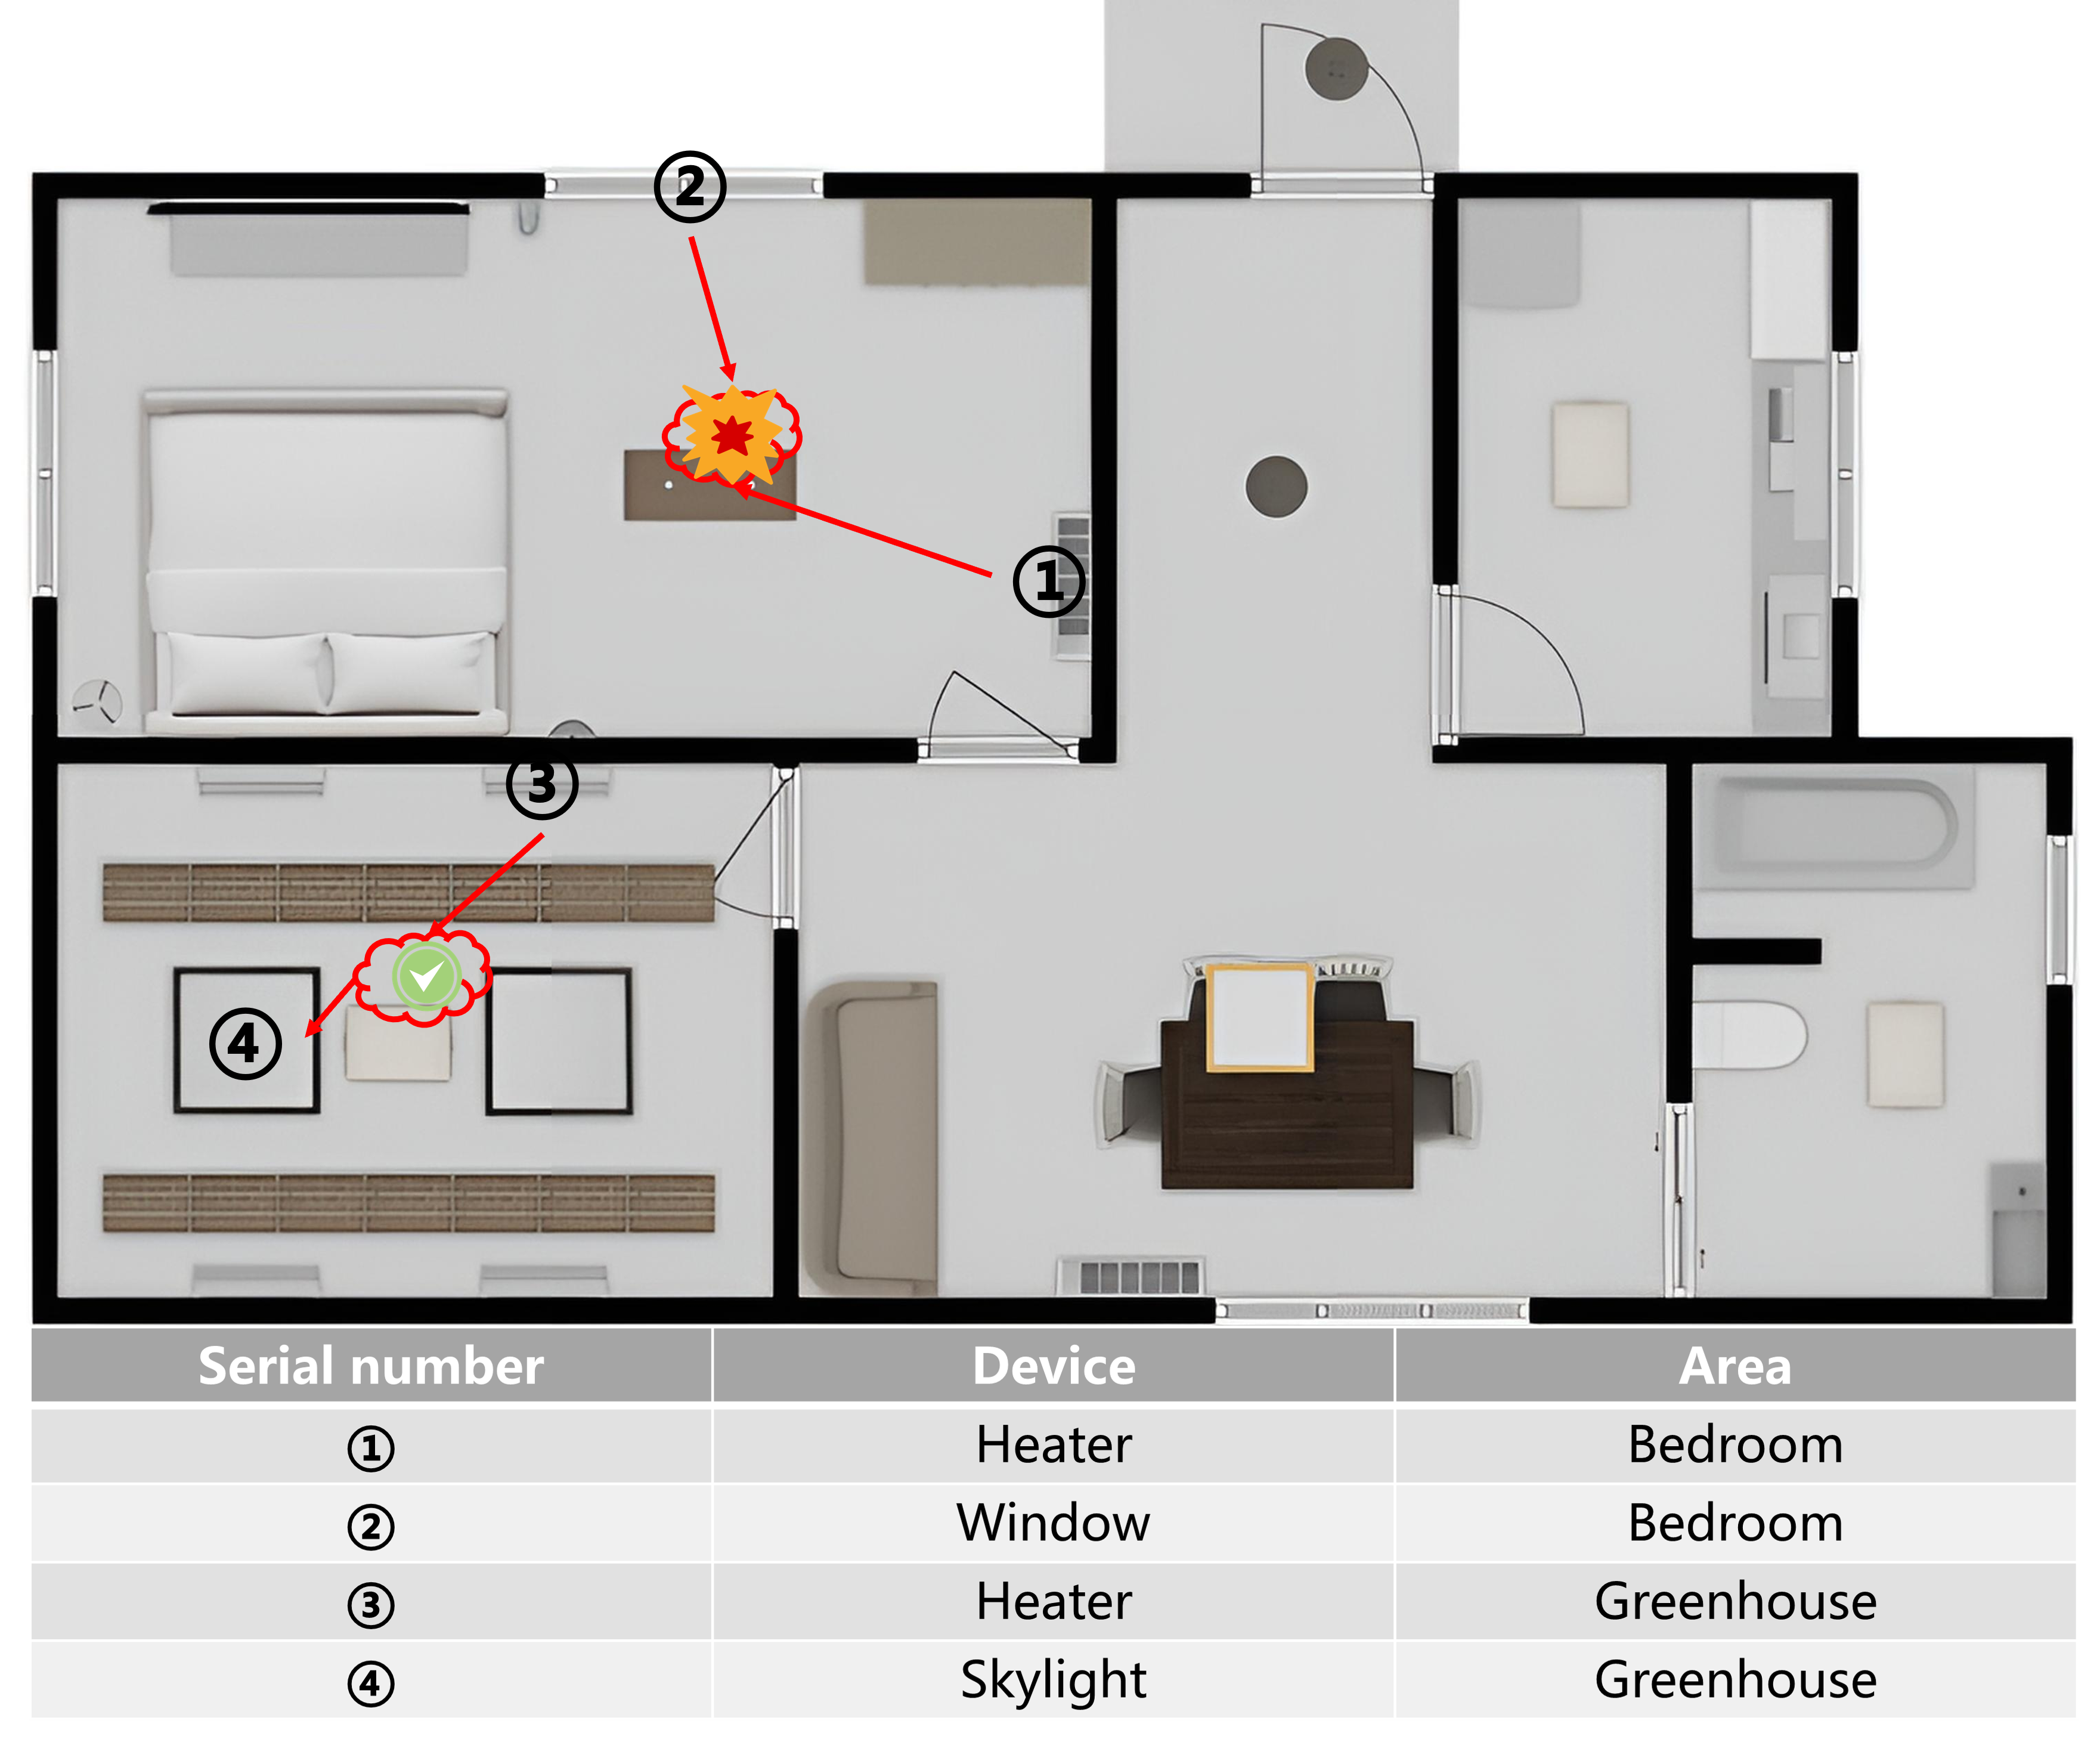
\includegraphics[width=0.4\textwidth]{figure/motivated_example.png}
	\caption{Motivating Example}
	\label{motivated_example}
\end{figure}

%本节提供了一个具体的例子来说明规则冲突的特征,并分析了现有冲突检测和缓解方法的局限性。图\ref{motivated_example}显示了一个智能家居的平面图,包括七个区域:室外(顶部中心)、门廊(中心)、客厅(底部中心)、厨房(右下)、浴室(右下)、卧室(左中心)和温室(左下)。\circled{1}是加热器,\circled{2}是卧室的窗户,\circled{3}是加热器,\circled{4}是温室的天窗。
This section provides a concrete example to illustrate the characteristics of rule conflicts and analyzes the limitations of existing conflict detection and mitigation methods. Figure \ref{motivated_example} shows a smart home floor plan including seven zones: outdoor (top center), porch (center), living room (bottom center), kitchen (bottom right), bathroom (bottom right), bedroom (left center), and greenhouse (bottom left). \circled{1} is a heater, \circled{2} is a bedroom window, \circled{3} is a heater, and \circled{4} is a greenhouse skylight.

% 请考虑以下在温室中设置的两条规则:规则 1 (R1):当检测到日落(触发条件)时,打开加热器(动作);规则 2 (R2):当温度达到 30 摄氏度时(触发条件),打开窗户并关闭加热器(动作)。
Consider the following two rules set in the greenhouse: Rule 1 (R1): When sunset is detected (trigger), turn on the heater (action); Rule 2 (R2): When the temperature reaches 30\celsius (trigger), open the window and turn off the heater (action).

\subsection{Challenge C1: Ambiguous Definition and Subjectivity of Rule Conflicts}


% 如图 \ref{motivated_example} 左下角所示,当 R1 和 R2 放置在温室中时,R1 的执行会加热温室。随着温度升高,R2 被触发,打开天窗并关闭加热器。在这种情况下,这种交互通常是预期的并且是功能性的。但是,如果这些规则应用于卧室(其中 \circled{2} 是卧室的窗户),R1 的执行会触发 R2,打开卧室的窗户。与温室天窗不同,在用户不知情的情况下自动打开卧室窗户可能会构成重大的安全风险,并且通常被认为是**意外后果**。这种差异,即使用相同的规则交互但根据环境和用户意图产生不同的结果,突出了规则冲突不仅仅基于交互模式本身,而是主观的,并且取决于用户的感知和安全问题。
As shown in the bottom left corner of Fig. \ref{motivated_example}, when R1 and R2 are placed in the greenhouse, the execution of R1 heats the greenhouse. As the temperature rises, R2 is triggered, opening the skylight and turning off the heater. In this context, this interaction is typically expected and functional. However, if these rules are applied to the bedroom (where \circled{2} is a bedroom window), R1's execution triggers R2, opening the bedroom window. Unlike a greenhouse skylight, opening a bedroom window automatically and without user knowledge can pose a significant security risk and is generally considered an **unintended consequence**. This discrepancy, using the same rule interaction but yielding different outcomes depending on the environment and user intent, highlights that rule conflicts are not solely based on the interaction pattern itself but are subjective and dependent on user perception and security concerns.

% 智能家居系统中规则冲突的定义缺乏统一标准。\cite{huang2023survey} 认为,并发的物联网规则执行可能导致意想不到的后果,并将此定义为规则冲突。然而,“意想不到的后果”涵盖范围广泛,包括明显的安全威胁以及用户未预料或不希望出现的结果。这种主观性使得仅根据规则的内在属性或交互模式来定义规则冲突具有挑战性。现有方法通常难以捕捉这种以用户为中心的方面,导致定义模糊,并且难以准确识别从用户角度来看真正有问题的冲突。发现和分类这些主观定义的“冲突”是一个重大挑战。
The definition of rule conflicts in smart home systems lacks a unified standard. \cite{huang2023survey} suggests that concurrent rule execution can lead to unintended consequences, defining this as a rule conflict. However, "unintended consequences" encompass a broad range, including clear security threats and outcomes simply unexpected or unintended by the user. This subjectivity makes it challenging to define rule conflicts solely based on intrinsic rule properties or interaction patterns. Existing methods often struggle to capture this user-centric aspect, leading to an ambiguous definition and difficulty in accurately identifying conflicts that are genuinely problematic from the user's perspective. Finding and categorizing these subjectively defined "conflicts" is a significant challenge.

% **我们的解决方案(S1):** 为了解决规则冲突的主观性并整合用户偏好,我们的方法采用了一种循序渐进的改进过程。我们首先对规则重新建模,结合用户家庭环境的特征,用户可以通过提供相关的区域信息来快速配置。随后,形式分析识别所有可能的规则互动。关键的是,我们接着使用用户提交的实体安全配置来自动识别违反这些安全策略的互动,并将它们标记为规则冲突。此外,用户保留根据特定互动的描述,手动指定一对规则互动是否根据他们的个人偏好构成冲突的能力。这种结合的方法允许基于已定义的安全标准的自动检测和基于主观偏好的用户驱动改进。
\textbf{Our Solution (S1):} To address the subjective nature of rule conflicts and integrate user preferences, our approach adopts a step-by-step refinement process. We begin by remodeling rules, incorporating characteristics of the user's home environment, which users can quickly configure by providing relevant region information. Subsequently, formal analysis identifies all possible rule interactions. Critically, we then use user-submitted entity security configurations to automatically identify interactions that violate these security policies, labeling them as rule conflicts. Furthermore, users retain the ability, based on the description of specific interactions, to manually designate whether a pair of rule interactions constitutes a conflict according to their personal preferences. This combined approach allows for both automated detection based on defined safety criteria and user-driven refinement based on subjective preference.

\subsection{Challenge C2: Diversity of Home Environments and Limited Generalization}

% 该示例进一步说明了智能家居环境的区域特性。虽然R1和R2在温室中可能是可以接受的,但它们在卧室中的应用(**图\ref{motivated_example} \circled{2} 卧室窗户**)会极大地改变其安全含义。这突出了相同的规则交互可能因特定设备、其位置和周围环境而产生不同的后果。现有的冲突检测方法仅依赖于规则结构或预定义的、固定的安全策略,难以应对这种多样性。为温室设计的安全策略(在温室中打开窗户可能没问题)不适用于卧室(在卧室中这是一种安全风险)。这种对特定家庭布局和设备配置的依赖需要高度定制化的策略。
The example further illustrates the regional characteristics of smart home environments. While R1 and R2 might be acceptable in the greenhouse, their application in the bedroom (**Fig. \ref{motivated_example} \circled{2} Bedroom Window**) drastically changes their safety implications. This highlights that the same rule interaction can have different consequences based on the specific device, its location, and the surrounding environment. Existing conflict detection methods relying solely on rule structure or predefined, fixed security policies struggle with this diversity. A security policy designed for the greenhouse (where opening a window might be fine) would not be applicable to the bedroom (where it's a security risk). This dependency on specific home layouts and device configurations requires highly customized strategies.

% 用户的家庭环境非常多样化,包括不同的布局、设备和用户期望。现有的基于固定安全策略的方法,虽然可能对特定设置中已知的冲突有效,但缺乏泛化能力。它们很难转移到不同的家庭环境,并且无法全面覆盖各种配置中无法预见的冲突。另一方面,仅依靠检测规则交互模式会产生大量误报(如温室示例),需要用户进行大量验证,并显着增加用户负担。设计一种在各种家庭环境中具有强大的泛化能力和准确性能的冲突检测和解决方案是一项重大挑战。“其他渠道”的影响,例如设备之间的空间关系(例如,门廊灯影响客厅亮度但不影响卧室亮度),增加了基于固定参数的检测通常会遗漏的另一层复杂性。
Users' home environments are highly diverse, encompassing varied layouts, devices, and user expectations. Existing methods based on fixed security policies, while potentially effective for known conflicts in specific setups, lack generalization ability. They are difficult to transfer to different home environments and cannot comprehensively cover unforeseen conflicts in diverse configurations. Relying solely on detecting rule interaction patterns, on the other hand, generates numerous false positives (like the greenhouse example), requiring substantial user effort for verification and significantly increasing the user burden. Designing a conflict detection and resolution scheme with strong generalization ability and accurate performance across various home environments is a significant challenge. The influence of "other channels," such as the spatial relationships between devices (e.g., porch lights affecting living room brightness but not bedroom brightness), adds another layer of complexity that fixed parameters-based detection often misses.

% **我们的解决方案 (S2):** 为了应对家庭环境的多样性并增强泛化能力,我们丰富了“侧信道”的概念,使其包括**区域、通道和趋势**。这种扩展的模型被纳入规则重新建模中。通过考虑环境的这些多方面因素,我们的方案能更有效地适应不同的用户设置。至关重要的是,我们没有采用固定的安全配置,而是利用用户提供的安全实体配置进行冲突检测,从而使该过程能够根据特定的家庭进行定制。在冲突解决方面,我们设计了多个可适应的策略模板,并按冲突类型进行分类。这些模板填充了特定的冲突信息,为根据每个已识别冲突的特征提供有针对性的解决方案选项。这种方法增强了方案在各种环境中进行泛化和准确执行的能力。
\textbf{Our Solution (S2):} To handle the diversity of home environments and enhance generalization, we enrich the concept of "side channels" to include **zone, channel, and trend**. This extended model is incorporated into rule remodeling. By considering these multi-faceted aspects of the environment, our scheme adapts more effectively to diverse user setups. Crucially, instead of fixed security configurations, we utilize user-provided security entity configurations for conflict detection, making the process tailored to the specific home. For conflict resolution, we design multiple adaptable strategy templates categorized by conflict types. These templates are populated with specific conflict information, providing targeted resolution options for each identified conflict based on its characteristics. This approach enhances the scheme's ability to generalize and perform accurately across varied environments.

\subsection{Challenge C3: Lack of User-Friendliness}

% 该示例表明,即使 R1 和 R2 之间看似简单的交互,也可能根据上下文产生复杂的影响。 向非技术用户解释这些细微差别和潜在风险可能很困难。 目前的方法通常以技术格式呈现冲突信息,或者要求用户手动定义复杂的安全策略。 对于卧室场景,仅仅被告知存在“触发交互”或“操作冲突”可能并不直观。 此外,解决方案可能涉及手动规则重新配置,正如尝试更改规则配置的示例所表明的那样,这可能很麻烦,无法实现所需的功能,甚至会引入新的冲突,需要专业的指导和大量用户的工作。 这种针对非专业用户的清晰度和易用性的缺乏是广泛采用的主要障碍。
The example demonstrates that even a seemingly simple interaction between R1 and R2 can have complex implications depending on context. Explaining these nuances and potential risks to a non-technical user can be difficult. Current methods often present conflict information in a technical format or require users to define complex security policies manually. For the bedroom scenario, simply being told there's a "Trigger Interaction" or "Action Conflict" might not be intuitive. Furthermore, resolution options might involve manual rule reconfiguration, which as the example of attempting to change rule configurations suggests, can be cumbersome, fail to achieve desired functionality, or even introduce new conflicts, requiring professional guidance and significant user effort. This lack of clarity and ease of use for non-expert users is a major barrier to widespread adoption.

% 目前,现有的规则冲突检测和解决方案缺乏用户友好性。基于规则交互模式的冲突检测会导致大量的误报,使用户被不相关的警报淹没(如温室误分类所示)。使用特定安全策略的方法难以在不同的家庭中推广,并且只能防止先前识别出的冲突。这两种方法都有缺点:用户工作量大、需要专家指导以及可扩展性有限。为非专业用户设计一种用户友好、高度自动化且易于实现的方案是一项紧迫的挑战。用户需要对潜在冲突的清晰解释和直接的解决方案选项,而无需深入的技术知识。
Current rule conflict detection and resolution schemes suffer from a lack of user-friendliness. Conflict detection based on rule interaction patterns leads to significant false positives, overwhelming users with irrelevant alerts (as seen in the greenhouse misclassification). Methods using specific security policies are difficult to generalize across different homes and can only prevent previously identified conflicts. Both approaches share drawbacks: high user workload, the need for expert guidance, and limited scalability. Designing a user-friendly, highly automated, and easily implemented scheme for non-professional users is a pressing challenge. Users need clear explanations of potential conflicts and straightforward options for resolution, without requiring deep technical knowledge.

% 我们的解决方案(S3): 为了应对用户友好性挑战,我们的方案在整个冲突检测和解决过程中优先考虑用户友好的界面。该界面引导用户提供必要的信息,例如他们的安全实体配置。当规则交互被自动识别为基于违反这些配置的冲突时,详细的冲突信息以易于理解的格式显示。然后,用户可以根据个人喜好从呈现的选项中选择冲突解决策略。此外,用户可以灵活地查看所有已识别的规则交互信息(以自然语言描述呈现),并为他们认为不希望的任何交互明确指定解决策略。所有冲突检测和解决过程都是自动化的,系统通过用户界面显示建议更改的优化自然语言描述。这种方法最大限度地减少了用户的工作量,消除了对日常任务的专家指导的需求,促进了个人偏好的配置,并且至关重要的是,保留了用户对决策的最终权限,使系统对非专业用户高度可访问和可用。
\textbf{Our Solution (S3):} To address the user-friendliness challenge, our scheme prioritizes a user-friendly interface throughout the conflict detection and resolution process. This interface guides users in providing necessary information, such as their security entity configurations. When rule interactions are automatically identified as conflicts based on violating these configurations, detailed conflict information is displayed in an easily understandable format. Users can then select conflict resolution strategies based on their personal preferences from the presented options. Additionally, users have the flexibility to review all identified rule interaction information (presented in natural language descriptions) and explicitly specify resolution strategies for any interaction they deem undesirable. All conflict detection and resolution processes are automated, with the system displaying optimized natural language descriptions of the proposed changes through the user interface. This approach minimizes user workload, eliminates the need for expert guidance for routine tasks, facilitates configuration of personal preferences, and crucially, retains the user's ultimate authority over decisions, making the system highly accessible and usable for non-professional users.

